%----------------------------------------------------------------------------------------
%    PACKAGES AND THEMES
%----------------------------------------------------------------------------------------
\documentclass[handout, aspectratio=169,xcolor=dvipsnames]{beamer}
\makeatletter
\def\input@path{{theme/}}
\makeatother
\usetheme{CleanEasy}
\usepackage[utf8]{inputenc}
\usepackage{lmodern}
\usepackage[T1]{fontenc}
% \usepackage[brazil]{babel}
\usepackage{fix-cm}
\usepackage{amsmath}
\usepackage{mathtools}
\usepackage{listings}
\usepackage{xcolor}
\usepackage{hyperref}
\usepackage{graphicx} % Allows including images
\usepackage{booktabs} % Allows the use of \toprule, \midrule and \bottomrule in tables
\usepackage{tikz}
\usetikzlibrary{positioning, shapes, arrows, calc, decorations.pathreplacing, arrows.meta, backgrounds, patterns, overlay-beamer-styles}
\usepackage{etoolbox}
\usepackage{animate}
\usepackage{multimedia}
\usepackage{media9}

\usepackage{subfiles}
\usepackage[normalem]{ulem}
\usepackage{cancel}
\usepackage{xmpmulti}
\newcommand{\bx}{\mathbf{x}}
\newcommand{\by}{\mathbf{y}}
\newcommand{\pd}{p_\text{data}}
\newcommand{\pt}{p_\theta}
\newcommand{\nbx}{\nabla_{\bx}}

\newcommand{\btx}{\mathbf{\tilde{x}}}
\newcommand{\qs}{q_{\sigma}}
\newcommand{\nbtx}{\nabla_{\btx}}

%----------------------------------------------------------------------------------------
%    LAYOUT CONFIGURATION
%----------------------------------------------------------------------------------------
\input{configs/configs}
%----------------------------------------------------------------------------------------

% References from references.bib
\usepackage[backend=bibtex,sorting=none]{biblatex}
\addbibresource{references.bib}


\begin{document}

\section{Week 6 Updates}

\begin{frame}{Summary}
    \begin{itemize}
        \item Fixed architecture from last meeting to be Lorentz-equivariant 
        \item Got exploding outputs (outliers on the order of $10^{20}$) under control
        \item Set up distributed training (HF accelerate)
        \item Fixed bug with scaling of jet attributes ($O(100-3000$ to $O(1)$ for all features))
        \item Continue to have issues with the model learning the trivial mapping
    \end{itemize}
\end{frame}

\begin{frame}[allowframebreaks]{Current architecture}
    \begin{enumerate}
        \item Embed scalar time value to random Fourier features through two fully connected layers with 32 and 64 nodes (following \cite{wuFastPointCloud2023})
        \item Concatenate time embedding with jet conditioning information, which consists of one-hot encoded type, $\eta$, mass, $p_T$, number of constituents
        \item Pass this through a fully connected layer of size 64 to produce the initial global embeddings $g^0$
        \item Concatenate $g^0$ with features $x_1^0 \dots x_N^0$ initialized from the initial distribution $p_0$.
        \item Now, we use $L$ Lorentz-group equivariant layers. \begin{enumerate}
            \item The input to the $l+1$-th layer is $g^l$ and $x^{l}_1 \dots x^l_N$.
            \item Calculate messages $m^l_{ij} = \phi_e^l(\psi(||x_i^l - x_j^l||), \psi(\langle x_i^l, x_j^l \rangle))$
            \item \textbf{Update the global embedding $$g_{l+1} = \phi^l_{g}(g^l, \alpha_l \sum\limits_{i, j \in [N]}  \phi_m^l(m_{ij}) \cancel{m^l_{ij})}$$}
            \item \textbf{Feed in the updated global embedding as well as the original embedding to update the graph embeddings} $$
            x_i^{l+1} = x_i^{l} + \gamma_l \sum\limits_{j \in N, j \neq i} \phi^l_{x} (g^0, g^{l+1}, m_{ij}) x_j^l
            $$
            \item Pass the results $g^{l+1}$ and $x_i^{l+1}$ to the next layer
        \end{enumerate}
        \item \textbf{Final output $v_\theta(t, x^0)_i = x_i^L \cancel{- x_i^{0}}$}
    \end{enumerate}

    \begin{itemize}
        \item $\phi$ = MLP with LeakyRELU activations except for $\phi_x$, which uses $\tanh$ (for expressiveness in linear combinations)
        \item $\alpha$ initialized to $\frac{1}{N^2}$, $\gamma$ initialized to $\frac{1}{N}$ 
    \end{itemize}
\end{frame}

\begin{frame}{Results}
    \begin{columns}
        \begin{column}{0.5\textwidth}
            \begin{figure}
                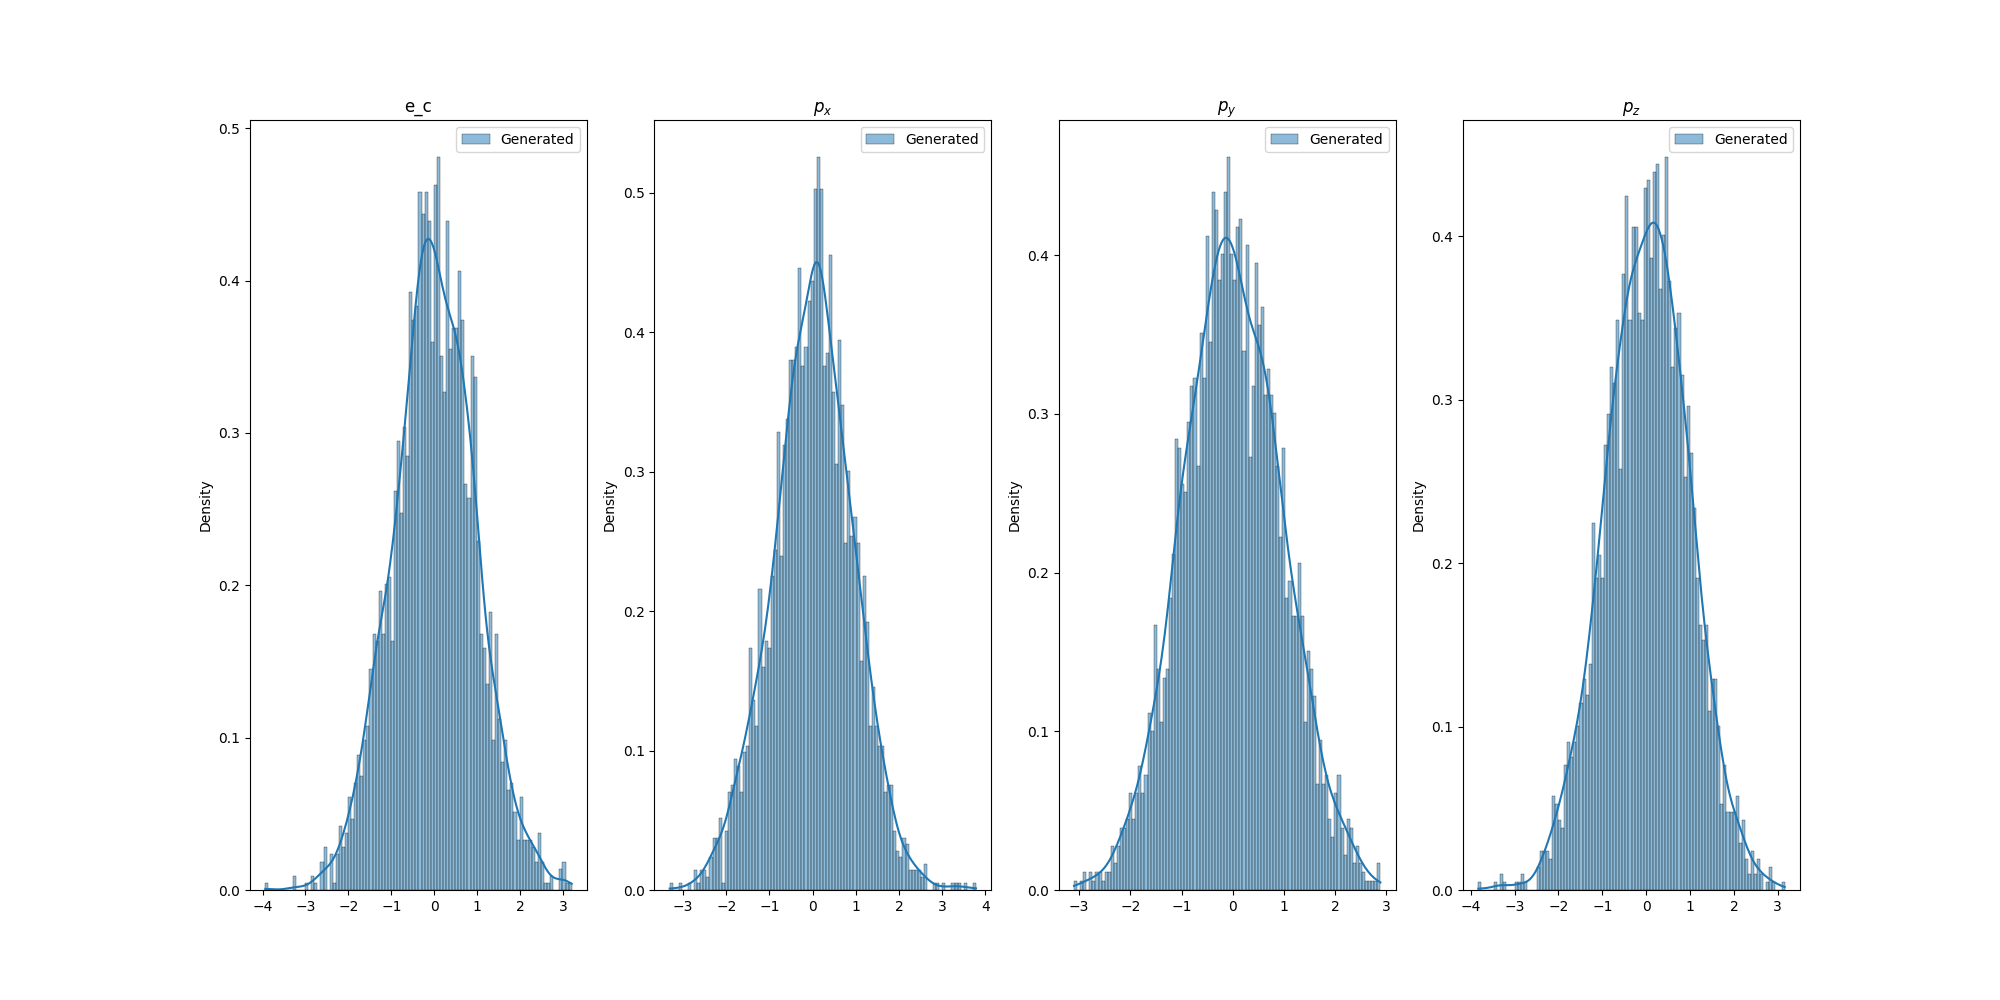
\includegraphics[width=\textwidth]{figs/week-6-results/lenetwork-final/samples_step-0.png}
            \end{figure}
        \end{column}
        \begin{column}{0.5\textwidth}
            \begin{figure}
                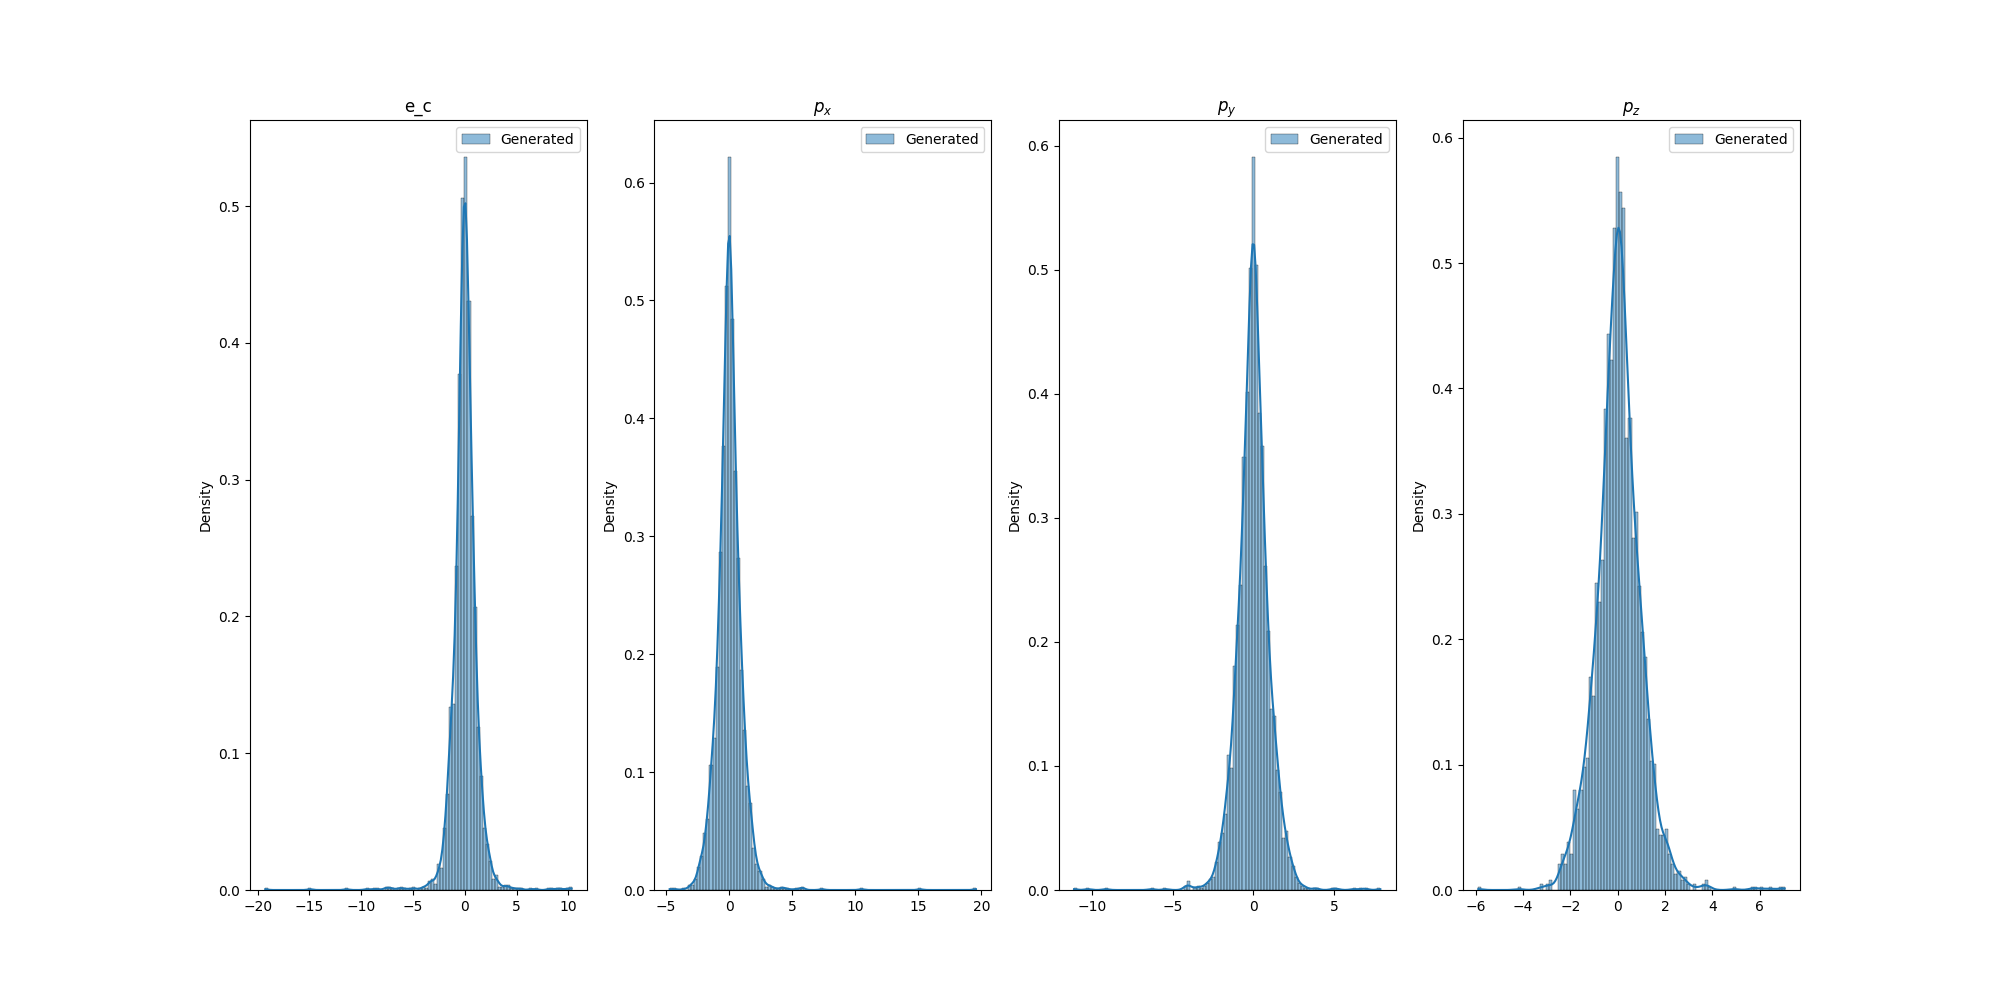
\includegraphics[width=\textwidth]{figs/week-6-results/lenetwork-final/samples_step-14.png}
            \end{figure}
        \end{column}
    \end{columns}
\end{frame}

\begin{frame}{Same results with simple, non-LE MLP}
    Only use time embedding and jet type to generate global embedding, pass through 6 layers with LeakyRELU actiations
    \begin{columns}
        \begin{column}{0.5\textwidth}
            \begin{figure}
                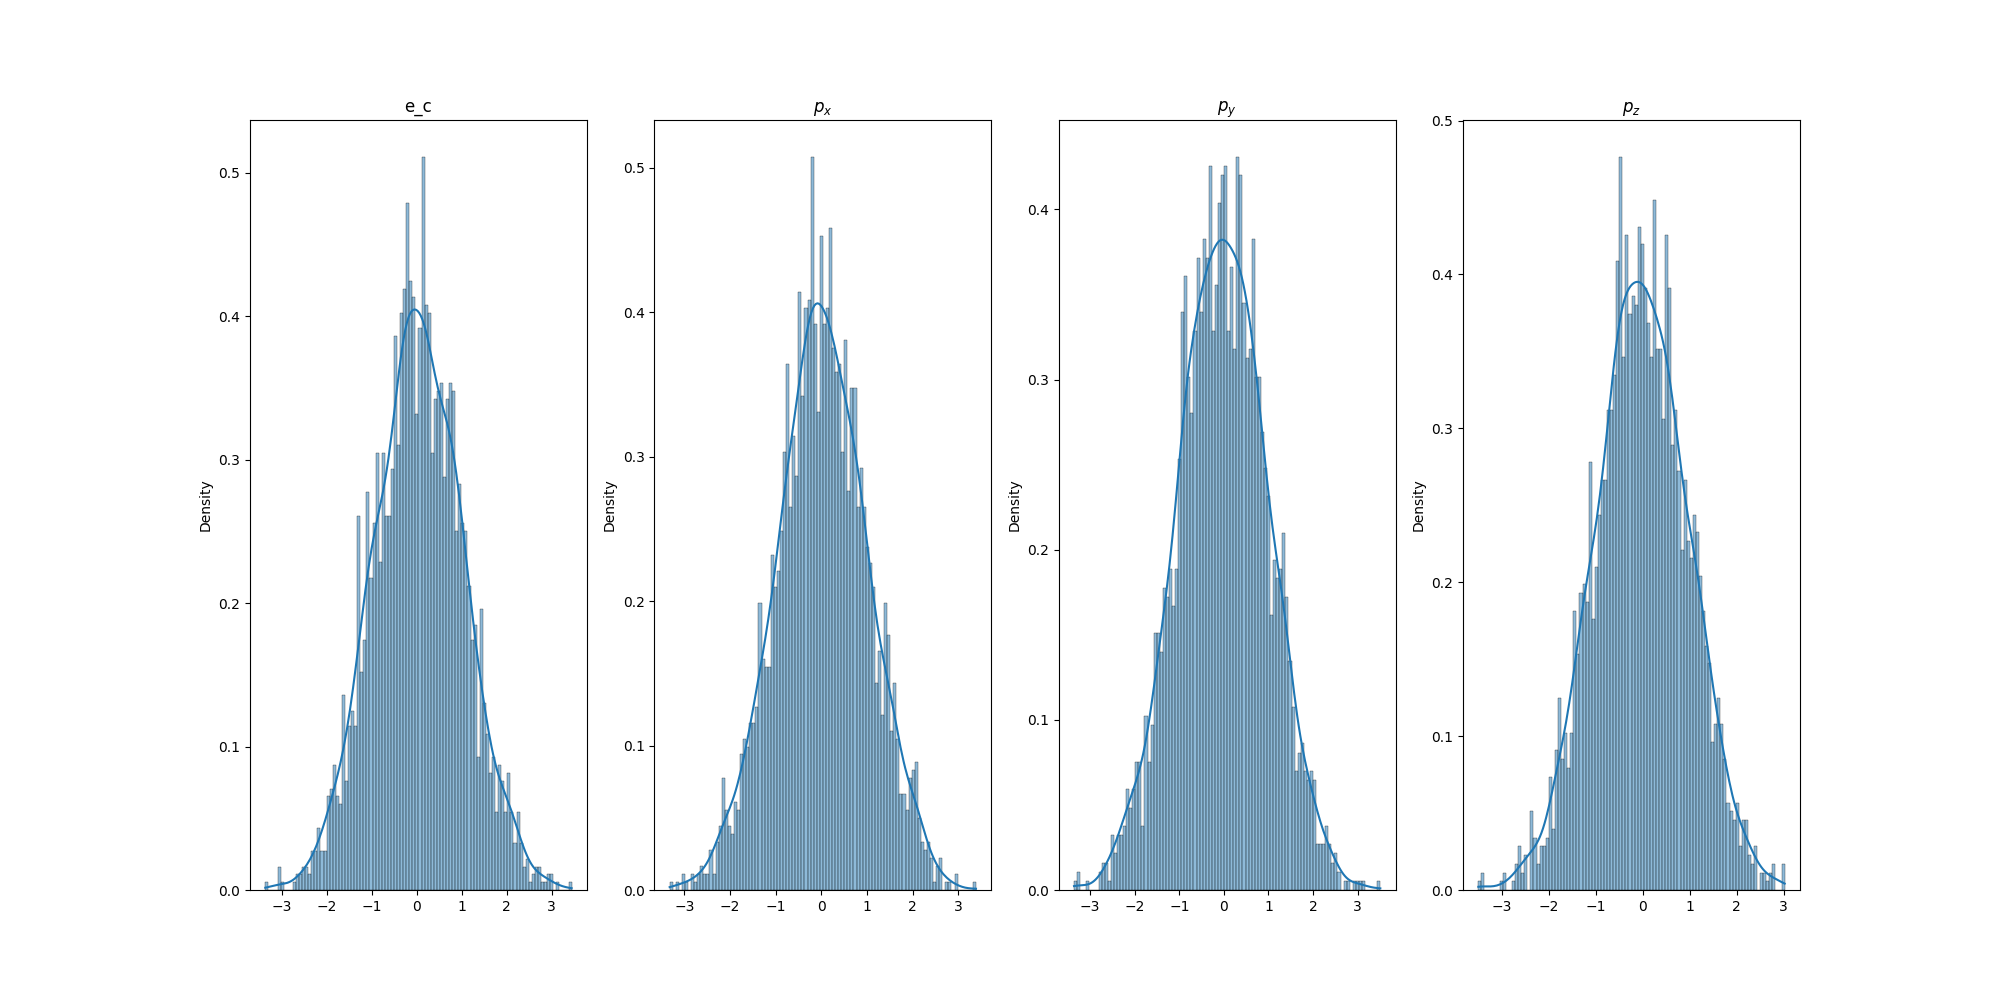
\includegraphics[width=\textwidth]{figs/week-6-results/mlp/samples_histogram_0001_step_0.png}
            \end{figure}
        \end{column}
        \begin{column}{0.5\textwidth}
            \begin{figure}
                
\includegraphics[width=\textwidth]{figs/week-6-results/mlp/samples_histogram_0001_step_15.png}
            \end{figure}
        \end{column}
    \end{columns}
\end{frame}

\begin{frame}{Train MLP only $E/c$}
    Maintain 150-dimensional particle cloud structure but discard $p_x, p_y, p_z$ in training
        \begin{columns}
        \begin{column}{0.5\textwidth}
            \begin{figure}
                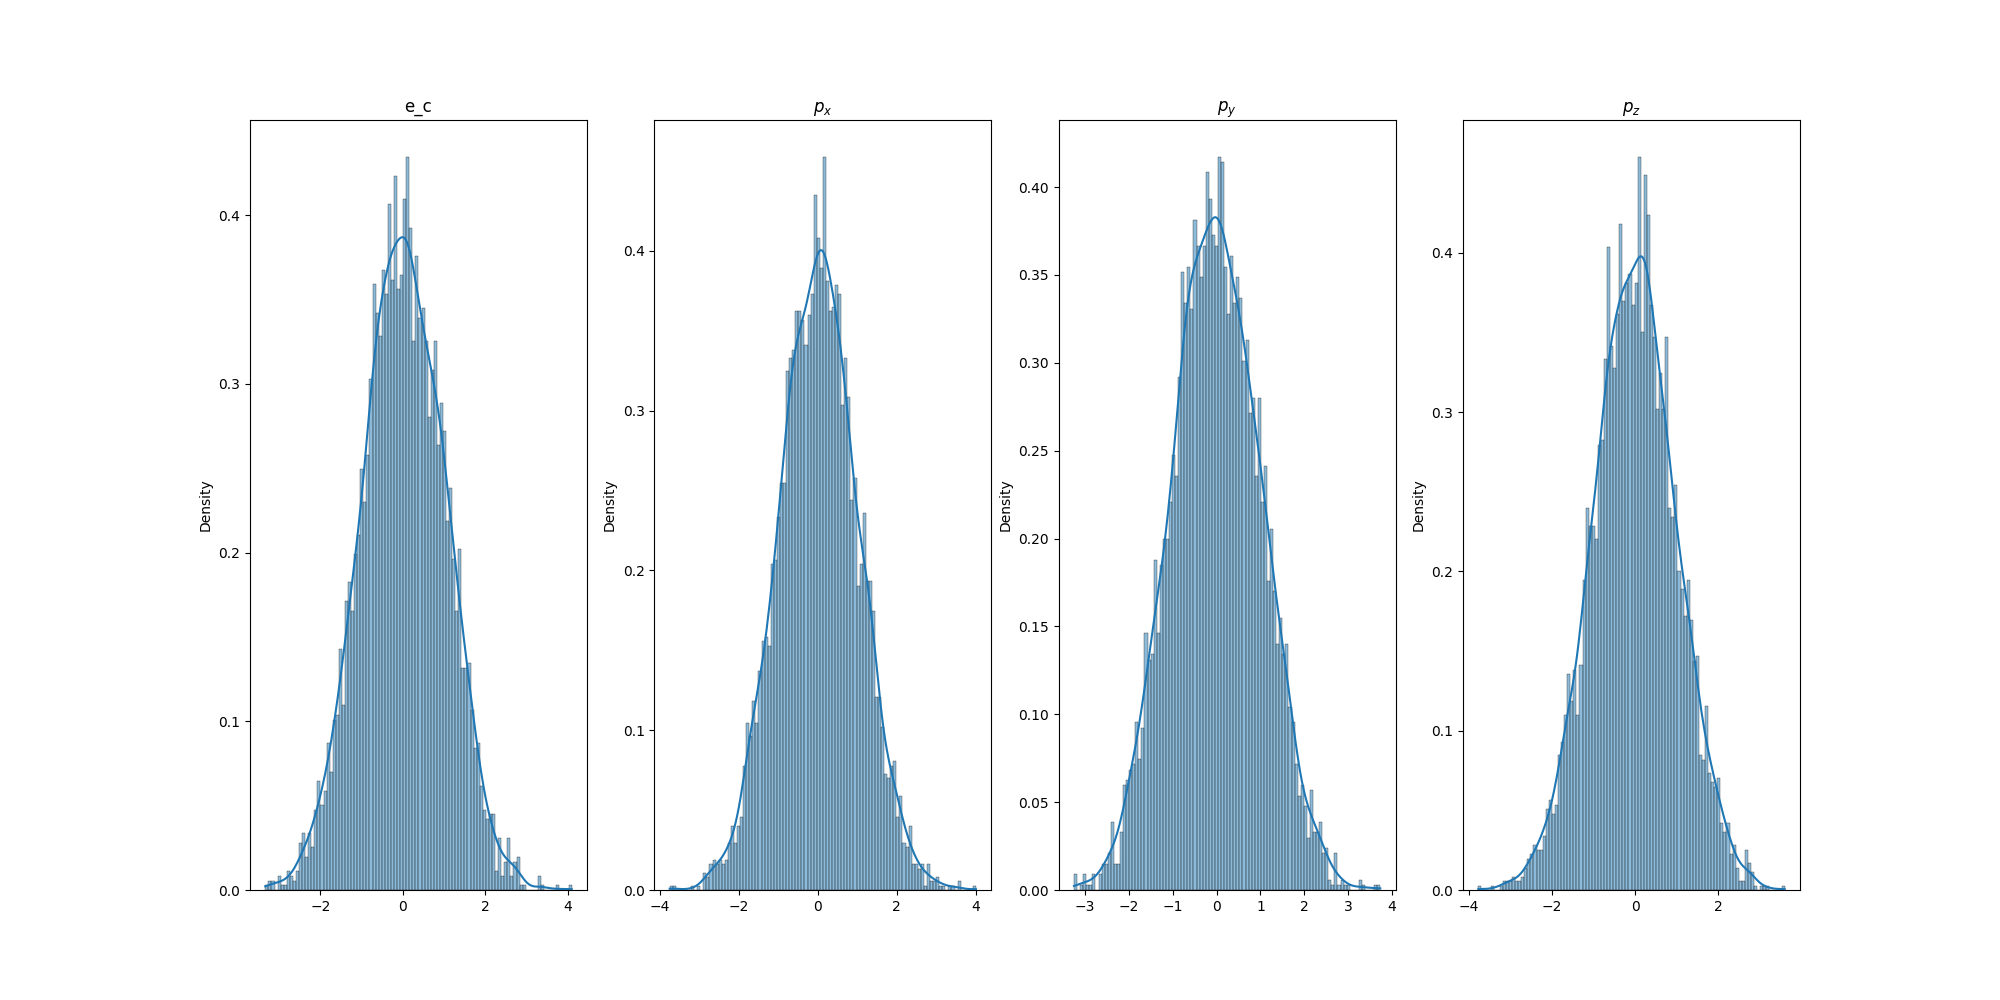
\includegraphics[width=\textwidth]{figs/week-6-results/mlp-only-ec/samples_histogram_0000_step_0.png}
            \end{figure}
        \end{column}
        \begin{column}{0.5\textwidth}
            \begin{figure}
                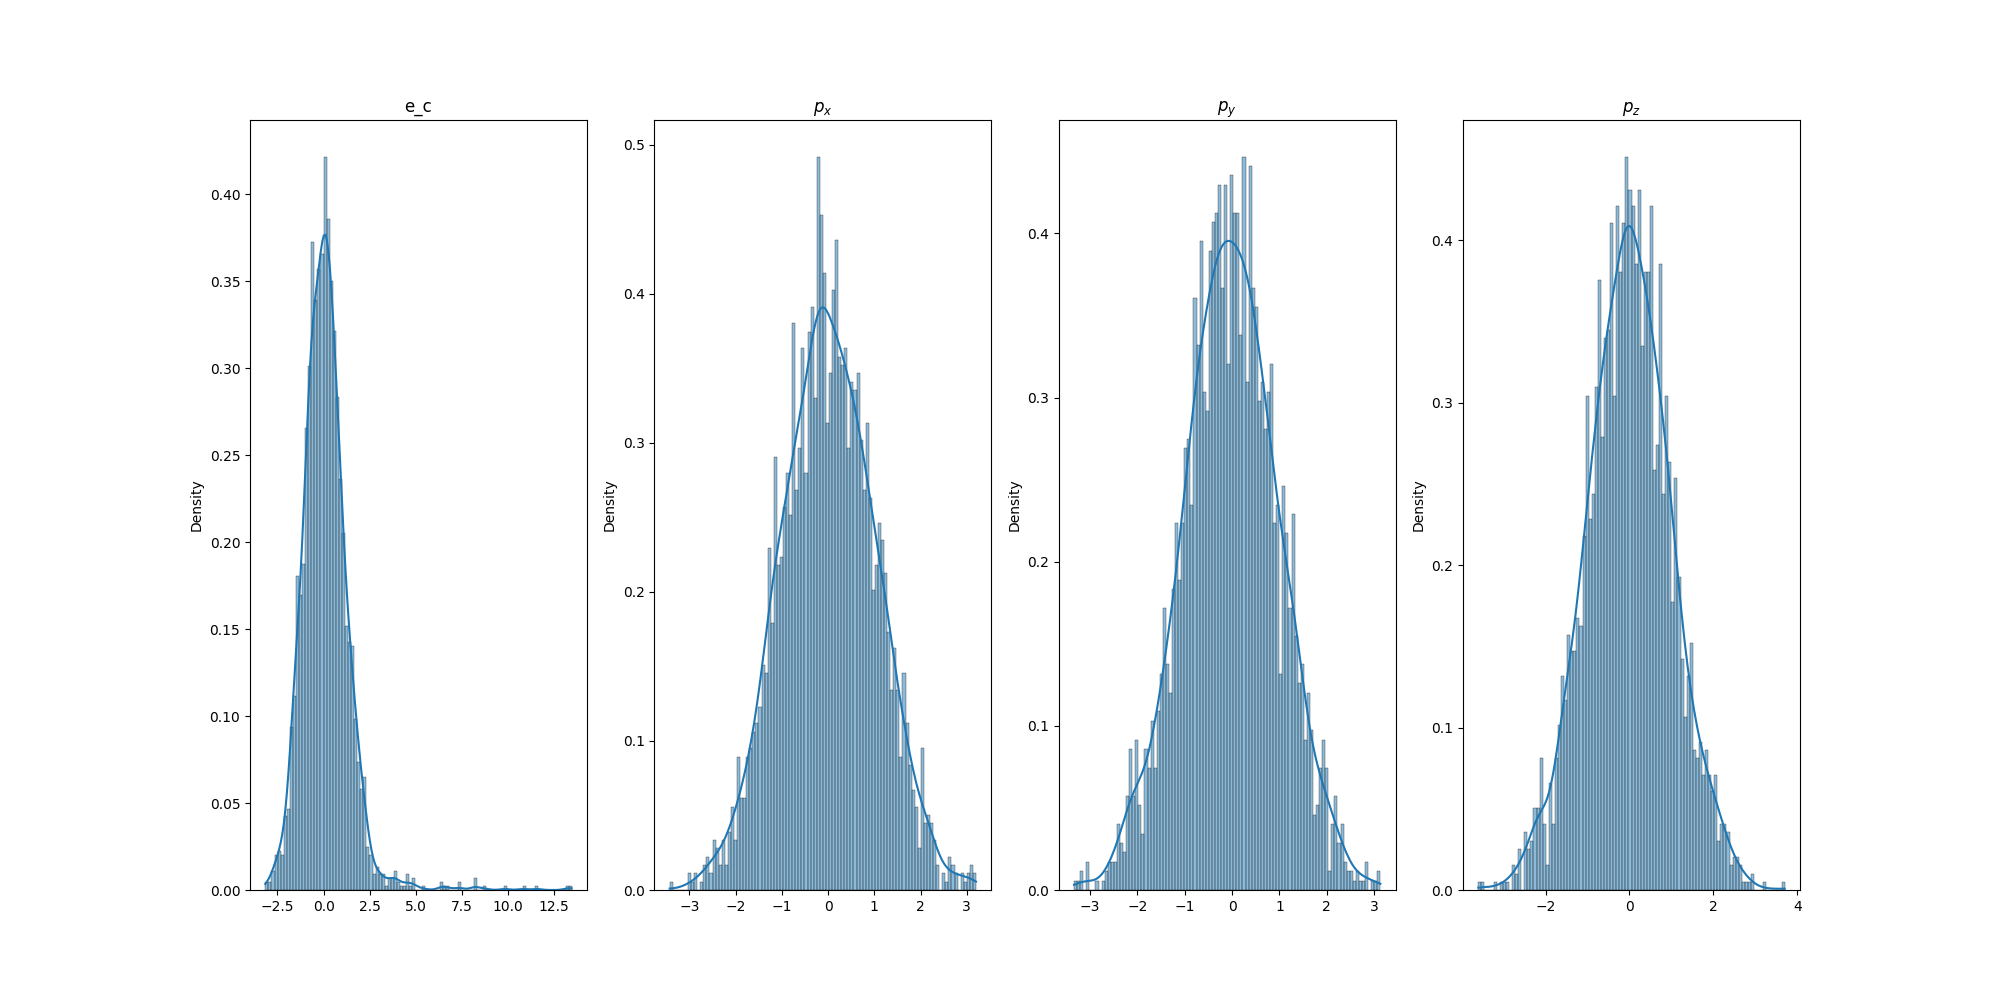
\includegraphics[width=\textwidth]{figs/week-6-results/mlp-only-ec/samples_histogram_0001_step_15.png}
            \end{figure}
        \end{column}
    \end{columns}
\end{frame}

\begin{frame}{Train unconditional MLP on 1-D flattened version of $E/c$}
    Remove jet attributes, flatten particle clouds (removing all zero-padded particles). Extract $5000~E/c$ values and train a simple MLP (from week 1)
    \begin{figure}
        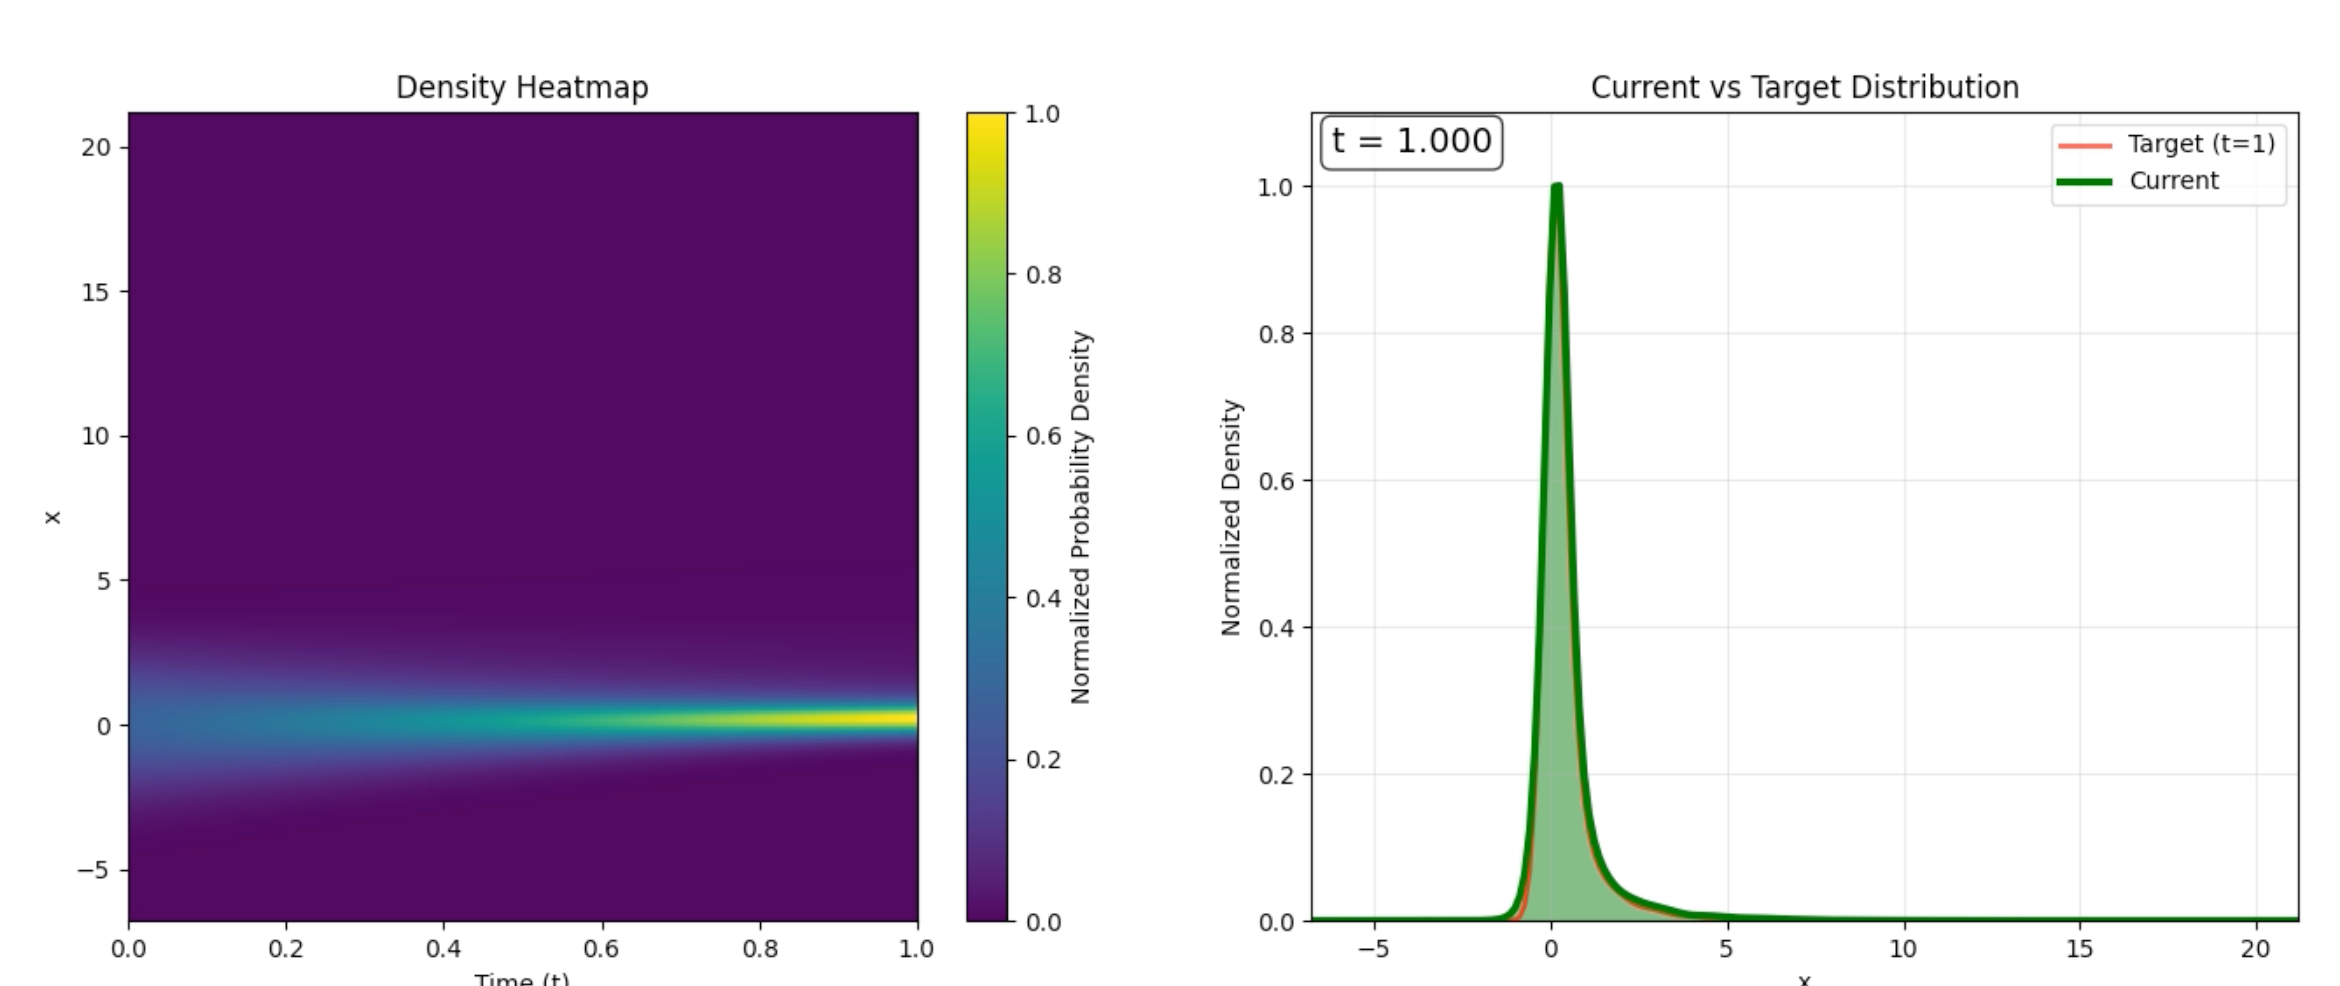
\includegraphics[height=0.6\textheight]{figs/week-6-results/simple-mlp-flat-ec.png}
    \end{figure}
\end{frame}

\begin{frame}{Hypotheses}
    \begin{itemize}
        \item Training difficulty or programming bugs with masking
        \item Time embedding not being transmitted through: updates are roughly the same for all timesteps
        \item \sout{Initial or intermediate particle clouds don't form a basis in 4-momenta space}
    \end{itemize}
\end{frame}

\begin{frame}{Ideas}
    \begin{itemize}
        \item Slightly refined architecture \begin{itemize}
            \item Transmit time embedding and global embedding separately, i.e., replace $g^L$ with $g^L, t_\text{emb}$ and $g^0$ with $g^0, t_\text{emb}$
            \item $m_{ij}^l = \phi_e^l (|| x_i^l - x_j^l||, \langle x_i^l, x_j^l \rangle, \mathbf{g^l, g^0})$
        \end{itemize}
        \item Break LE in the last step \begin{itemize}
            \item LorentzNet stacks LE blocks but at the end, uses average pooling $\rightarrow$ dropout $\rightarrow$ decoding layer $\rightarrow$ softmax
            \item Eg. $v_\theta(t, x_0)_i = \phi_{out}([g_0 \text{ or } t], g^L, x_i^L, x_i^0)$
        \end{itemize}
        \item Have multiple message-passing steps in the same layer, i.e., repeat $x_i^{l+1} = x_i^{l} + \gamma_l \sum\limits_{j \in N, j \neq i} \phi^l_{x} (g^0, g^{l+1}, m_{ij}) x_j^l$ inside a layer
        \item Linear combination with differences between 4-vectors based on E(3) GNN \cite{satorrasEquivariantGraphNeural2022a} $$x_i^{l+1} = x_i^l + \sum\limits_{j \neq i} \phi_x^l(g^0, g^{l+1}, m_{ij}) \mathbf{\frac{x_i^l - x_j^l}{||x_i^l - x_j^l|| + 1}} $$
    \end{itemize}
\end{frame}

\begin{frame}{Potential refinements}
    \begin{itemize}
        \item Using simple linear conditional flow objective (theoretically best for training stability), could try more sophisticated affine flows \cite{lipmanFlowMatchingGuide2024} or DDIM (theoretically less stable)
        \item Currently 16 Euler integration steps, 128-512 is more typical in published work (tend to get diminishing returns)
        \item Increased batch size: currently restricted to $\approx$ 50 with $\mathcal{O}(N^2)$ network on particle clouds with $N_C=150$ (on a 24 GB device)
    \end{itemize}
    But none of these should be the difference between trivial and meaningful output 
\end{frame}


\begin{frame}{Pending fixes}
    \begin{itemize}
        \item Global features (jet $\eta$, $m$, $p_T$, \# constituents) are \begin{enumerate}
            \item Produced with a non-LE normalizing flow
            \item Are passed through an MLP (with time embedding and one-hoot encoded jet type) in the main flow matching network to produce the global embedding, which breaks LE
        \end{enumerate}
        Potential fix: only generate LE feature (\# constituents) as part of the global embedding
        \item Discussion from last week on the initial distribution - using a simple normal right now for debugging (not LE)
    \end{itemize}
\end{frame}

\begin{frame}[allowframebreaks]{New architecture}
    \begin{enumerate}
        \item Embed scalar time value to random Fourier features through two fully connected layers with 32 and 64 nodes (following \cite{wuFastPointCloud2023}) to produce $t_\text{emb}$
        \item Pass jet information (one-hot encoded jet type and scalar number of jet constituents $N_C$) through 2 fully connected layers to 64-dimensional embedding $g_0$
        \item Pass this through a fully connected layer of size 64 to produce the initial global embeddings $g^0$
        \item Concatenate $g^0$ with features $x_1^0 \dots x_N^0$ initialized from the initial distribution $p_0$.
        \item Now, we use $L$ Lorentz-group equivariant layers. \begin{enumerate}
            \item The input to the $l+1$-th layer is $g^l$ and $x^{l}_1 \dots x^l_N$.
            \item Calculate messages $m^l_{ij} = \phi_e^l(\psi(||x_i^l - x_j^l||), \psi(\langle x_i^l, x_j^l \rangle))$
            \item \textbf{Update the global embedding $$g_{l+1} = \phi^l_{g}(g^l, \alpha_l \sum\limits_{i, j \in [N]}  \phi_m^l(m_{ij}) \cancel{m^l_{ij})}$$}
            \item \textbf{Feed in the updated global embedding as well as the original embedding to update the graph embeddings} $$
            x_i^{l+1} = x_i^{l} + \gamma_l \sum\limits_{j \in N, j \neq i} \phi^l_{x} (g^0, g^{l+1}, m_{ij}) x_j^l
            $$
            \item Pass the results $g^{l+1}$ and $x_i^{l+1}$ to the next layer
        \end{enumerate}
        \item \textbf{Final output $v_\theta(t, x^0)_i = x_i^L \cancel{- x_i^{0}}$}
    \end{enumerate}

    \begin{itemize}
        \item $\phi$ = MLP with LeakyRELU activations except for $\phi_x$, which uses $\tanh$ (for expressiveness in linear combinations)
        \item $\alpha$ initialized to $\frac{1}{N^2}$, $\gamma$ initialized to $\frac{1}{N}$ 
    \end{itemize}
\end{frame}



\begin{frame}[allowframebreaks]{References}
\printbibliography
\end{frame}
\end{document}
